\section{Execution of unmodified guest OS's}
Execution of unmodified guest OS’s is done through a
process called binary conversion. Emulation of one
processing architecture over another is accomplished with
this technology. By simulating one instruction set after
another through code translation, it enables the execution
of unaltered guest operating systems. QEMU \cite{citation_13}, a
processor emulator created by Fabrice Bellard, is an
illustration of multiplatform emulation. Although further
architectures are being developed, QEMU now supports
full CPU emulation of x86, x86-64, ARM, SPARC,
PowerPC, MIPS, and m68k (Coldfire) \cite{citation_14}. In other
words, QEMU may run operating systems that were
initially designed for these processors. These days,
QEMU is available for Linux, Windows, Mac OS X, and
OpenSolaris, and it supports all host CPUs, including
x86, x86-64, and PowerPC. The flexibility to migrate
application code and operating systems across platforms
is a benefit of full processor emulation; however, the
overhead resulting from simulating the entire instruction
set is a drawback.
\begin{figure}[h]
    \centering
    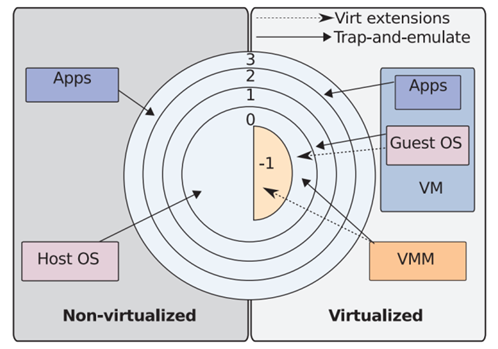
\includegraphics[width=\linewidth]{./images/cpu-protection-rings.png}
    \caption{CPU protection rings}
    \label{fig:cpu_protection_rings}
\end{figure}
\newline
Virtualisation also makes use of binary translation. The
goal of virtualization, having replica of virtual machines
of the real machine, is accomplished by combining binary
translation with direct execution. BT is used to translate
or simulate a limited set of CPU instructions, in contrast
to emulation. That is, code like kernel-mode and real
mode that requires privileged execution (Ring 0). The
host CPU carries out the remaining instructions directly.
VMware virtualisation solutions \cite{citation_15} and QEMU
Accelerator (KQEMU) \cite{citation_16} are two examples that make
use of comparable methods. This method exhibits low
overhead and performs better than full emulation.
However, unlike emulation, only guest operating systems
that operate within the host CPU are supported. \newline \newline
The idea of hardware-assisted virtualisation is not new.
When the Virtual Machine Facility for the IBM System
became available in 1972, it was first put into practice
\cite{citation_1}. Recently, in 2006, chip manufacturers like AMD and
Intel included virtualisation to their products. Figure \ref{fig:cpu_protection_rings}
showcases how hardware-assisted virtualisation creates a
Ring with a higher privileged mode in the processor
architecture. Unmodified guest operating systems can run
in Ring 0, non-root mode, and the VMM or Hypervisor in
Ring -1, root mode, thanks to CPU extensions for
virtualisation support. By improving CPUs, hardwareassisted virtualisation enables virtualisation without
requiring binary translation or para-virtualization. The
benefit of this strategy is that it uses hardware rather than
software to alleviate the overhead brought on by the trapand-emulate model. Kernel-based virtual machines
(KVM) such as, VirtualBox, Xen, Hyper-V, and VMware
products are a few examples of hardware-assisted
virtualisation.